\section{Methodology}
\label{sec:method}

\subsection{Problem Setting and Overview}

Let $X=\{(t_j,\mathbf{x}_j,\mathbf{m}_j)\}_{j=1}^{L}$ be an
irregular multivariate history. Index $j$ denotes a history event on the union
of observed timestamps, $\mathbf{x}_j\in\mathbb{R}^{D}$ stores the sensor
values at that event, and $\mathbf{m}_j\in\{0,1\}^{D}$ indicates which values
are observed. Given future query times $\{t_h^+\}_{h=1}^{H}$, the model
predicts $\widehat{\mathbf y}_h\in\mathbb{R}^{D}$. Future availability masks
are used only by the loss and evaluator.

Figure~\ref{fig:v665-framework} gives the complete forward path. MESANet first
canonicalizes each sample--variable history using observed entries. It then
builds two patch sequences: a low-frequency coordinate $\mathbf L$ retaining
fixed and multiresolution support evidence, and an ordered waveform coordinate
$\mathbf W$ retaining within-patch values, masks, and first differences.
Coordinate-specific representations produce low- and high-frequency forecasts.
A bounded projection controls their subspace overlap before affine restoration.

\begin{figure*}[t]
\centering
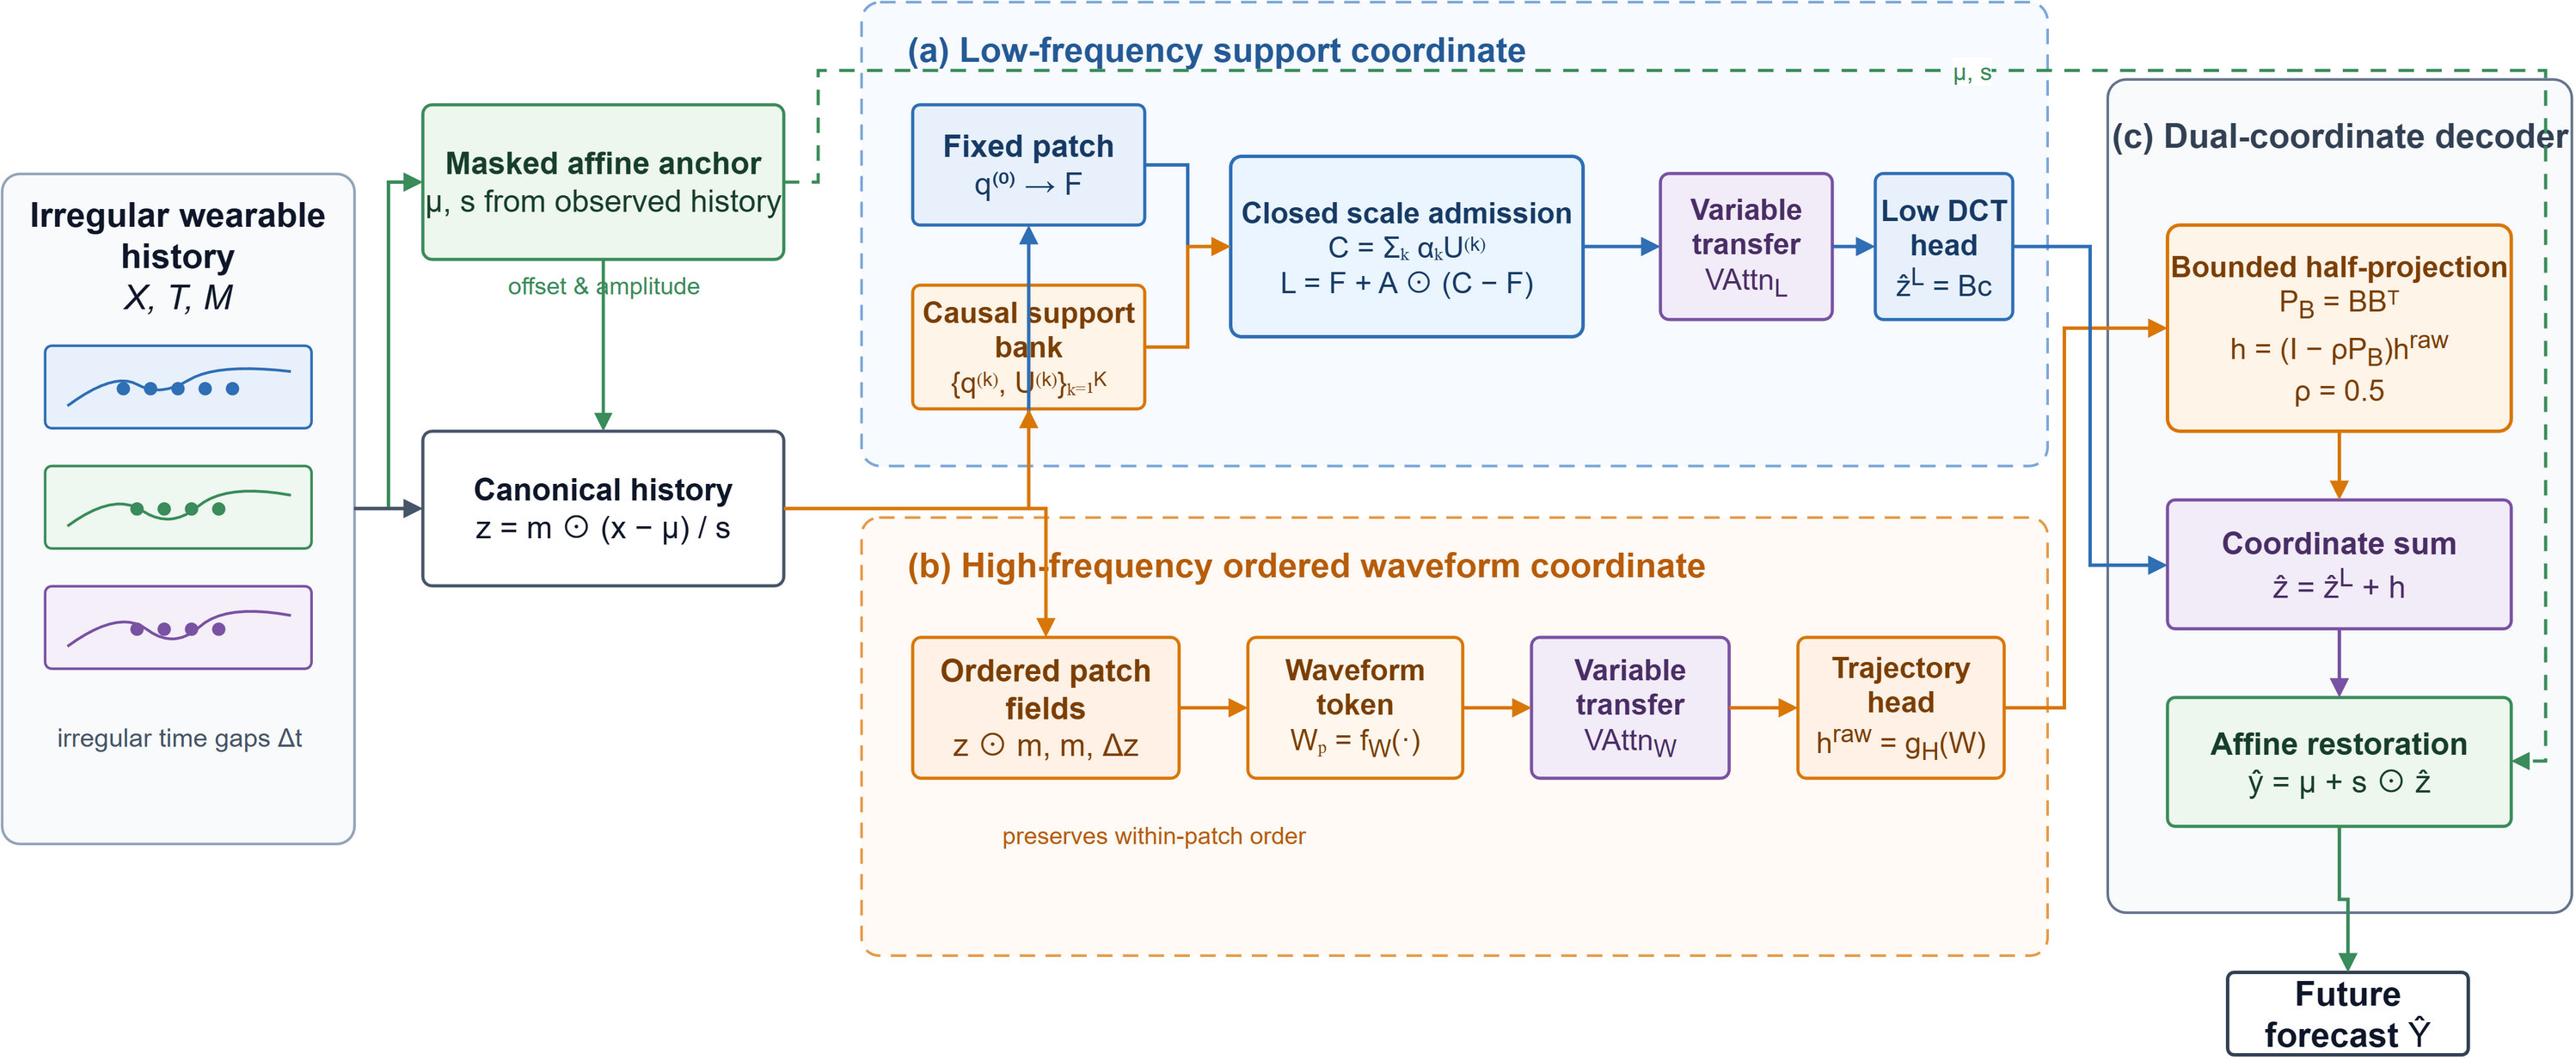
\includegraphics[width=\textwidth]{figures/final/mesa_fig2_v676.png}
\caption{MESANet architecture. Masked affine anchoring feeds a low-frequency
support coordinate and an ordered waveform coordinate. Coordinate-specific
variable transfer and forecast heads are combined by bounded DCT-subspace
separation before affine restoration.}
\label{fig:v665-framework}
\end{figure*}

\subsection{Masked Affine Anchoring}

For sample $b$ and variable $i$, the number of observed history values, their
mean, and their scale are
\begin{align}
n_{bi} &= \sum_{j=1}^{L}m_{bji}, \label{eq:count}\\
\mu_{bi} &= \frac{\sum_jm_{bji}x_{bji}}{\max(n_{bi},1)}, \label{eq:mean}\\
s_{bi} &= \max\!\left(
\sqrt{\frac{\sum_jm_{bji}(x_{bji}-\mu_{bi})^2}{\max(n_{bi},1)}+\epsilon},
s_{\min}\right). \label{eq:scale}
\end{align}
When $n_{bi}=0$, we use $(\mu_{bi},s_{bi})=(0,1)$. The canonical history is
\begin{equation}
z_{bji}=m_{bji}\frac{x_{bji}-\mu_{bi}}{s_{bi}},
\label{eq:canonical}
\end{equation}
and the final normalized forecast $\widehat z_{bhi}$ is restored by
\begin{equation}
\widehat y_{bhi}=\mu_{bi}+s_{bi}\widehat z_{bhi}.
\label{eq:restore}
\end{equation}
The anchor keeps offset and amplitude outside the learned dynamics while masks
prevent unobserved placeholders from entering its statistics.

\subsection{Low-Frequency Support Coordinate}

Let $\tau_p$ be the right boundary of patch $p$ and $I_p$ its fixed causal
interval. The fixed branch summarizes observed canonical values in $I_p$ using
density, nonempty support, mean, variance, first and last values, local slope,
observed span, recency, and the patch center. We denote this history-only
statistic by $\mathbf q^{(0)}_{bip}$. A fixed encoder with patch-time and
variable embeddings forms
\begin{equation}
\mathbf F_{bip}=f_F\!\left(
[\mathbf q^{(0)}_{bip},\operatorname{TE}(\tau_p),\mathbf e_i]\right).
\label{eq:fixed-token}
\end{equation}
Here, $\operatorname{TE}(\tau_p)$ is the patch-time embedding, $\mathbf e_i$
is the learned variable embedding, and $f_F$ is the fixed-coordinate encoder.

In parallel, $K$ causal exponential supports retain alternative ranges. For a
learnable positive width $w_k$, observation $j$ receives
\begin{align}
r^{(k)}_{bipj} &=m_{bji}\mathbf 1[t_j\leq\tau_p]
\exp\!\left(-\frac{\tau_p-t_j}{w_k+\epsilon}\right), \label{eq:support-weight}\\
\omega^{(k)}_{bipj} &=
\frac{r^{(k)}_{bipj}}{\sum_{\ell}r^{(k)}_{bip\ell}+\epsilon}.
\label{eq:normalized-weight}
\end{align}
The same statistic fields are recomputed with $\omega^{(k)}$, producing
$\mathbf q^{(k)}_{bip}$ and token $\mathbf U^{(k)}_{bip}$. Thus every support
describes the same variable and anchor but uses a different causal range. A
history-state score selects their mixture:
\begin{align}
\ell^{(k)}_{bip} &= f_\alpha(\mathbf q^{(k)}_{bip},\tau_p,\mathbf e_i)
+ b_k(\mathbf q^{(0)}_{bip}), \label{eq:scale-logit}\\
\alpha^{(k)}_{bip} &=
\frac{\exp(\ell^{(k)}_{bip})}{\sum_{r=1}^{K}\exp(\ell^{(r)}_{bip})},
\label{eq:scale-softmax}\\
\mathbf C_{bip} &= \operatorname{LN}\!\left(
\sum_{k=1}^{K}\alpha^{(k)}_{bip}\mathbf U^{(k)}_{bip}+\mathbf e_i\right).
\label{eq:scale-token}
\end{align}
Here and below, $\operatorname{LN}$ denotes layer normalization.

A bounded vector-valued admission map uses the fixed and scale statistics and tokens:
\begin{align}
\mathbf A_{bip} &= \sigma\!\left(f_A(\mathbf F_{bip},\mathbf C_{bip},
\mathbf q^{(0)}_{bip},\textstyle\sum_k\alpha^{(k)}_{bip}\mathbf q^{(k)}_{bip})
\right), \label{eq:admission}\\
\mathbf L_{bip} &= \operatorname{LN}\!\left(
\mathbf F_{bip}+\mathbf A_{bip}\odot(\mathbf C_{bip}-\mathbf F_{bip})\right).
\label{eq:level-token}
\end{align}
Since $\mathbf A_{bip}\in(0,1)^d$, each pre-normalization dimension lies
between its fixed and multiresolution values. The low-frequency branch can
therefore admit longer support without an unrestricted additive correction.

\subsection{Ordered Waveform Coordinate}

Summary statistics in Eq.~\eqref{eq:fixed-token} intentionally suppress
within-patch order. MESANet preserves that order in a separate field. For the
$P$ positions assigned to patch $p$, let $\mathbf z_{bip}\in\mathbb R^P$ and
$\mathbf m_{bip}\in\{0,1\}^{P}$ be the canonical values and masks. The masked
first difference is
\begin{equation}
\begin{aligned}
\Delta\mathbf z_{bip}[r] ={}&
\mathbf m_{bip}[r]\mathbf m_{bip}[r-1] \\
&\cdot(\mathbf z_{bip}[r]-\mathbf z_{bip}[r-1]),\quad r>1,
\end{aligned}
\label{eq:wave-diff}
\end{equation}
with zero at $r=1$. The ordered waveform token is
\begin{equation}
\mathbf W_{bip}=f_W\!\left(
[\mathbf z_{bip}\odot\mathbf m_{bip},\mathbf m_{bip},
\Delta\mathbf z_{bip},\mathbf e_i]\right).
\label{eq:wave-token}
\end{equation}
Unlike $\mathbf q^{(k)}$, this vector is sensitive to the ordering of observed
motion inside a patch. Masks distinguish an actual zero from an unavailable
position, while first differences expose local velocity without replacing the
level coordinate.

\subsection{Dual-Coordinate Forecasting}

MESANet retains separate support and waveform representations through variable
interaction. In the default implementation, scaled dot-product attention is
applied to each coordinate at every patch:
\begin{align}
\widetilde{\mathbf L}_{bp} &=
\operatorname{VAttn}_L(\mathbf L_{bp}), \label{eq:level-transfer}\\
\widetilde{\mathbf W}_{bp} &=
\operatorname{VAttn}_W(\mathbf W_{bp}). \label{eq:wave-transfer}
\end{align}
The operators $\operatorname{VAttn}_L$ and $\operatorname{VAttn}_W$ are
scaled dot-product attention across variables for the support and waveform
coordinates, respectively.
This coordinate-specific parameterization preserves the branch identities.
The factorization concerns the representations and forecast geometry, not a
requirement that their transfer parameters be disjoint; Section~\ref{sec:ablation}
therefore includes an equal-capacity shared-transfer control.

Let $\mathbf B\in\mathbb R^{H\times R}$ contain the first $R$ orthonormal
discrete-cosine basis vectors, where $R\ll H$. A low head maps the ordered
level-token trajectory to coefficients $\mathbf c_{bi}\in\mathbb R^R$:
\begin{align}
\mathbf c_{bi} &= g_L(\operatorname{vec}\{\widetilde{\mathbf L}_{bip}\}_{p=1}^{P}),
\label{eq:low-coeff}\\
\widehat{\mathbf z}^{L}_{bi} &= \mathbf B\mathbf c_{bi}.
\label{eq:low-forecast}
\end{align}
The waveform head directly predicts an $H$-step trajectory
\begin{equation}
\mathbf h^{\rm raw}_{bi}=g_H(
\operatorname{vec}\{\widetilde{\mathbf W}_{bip}\}_{p=1}^{P}).
\label{eq:raw-high}
\end{equation}
To avoid both unconstrained duplication and exact orthogonality, MESANet uses
the fixed bounded separation strength $\rho=1/2$ and applies
\begin{align}
\mathbf P_B &= \mathbf B\mathbf B^\top, \label{eq:projector}\\
\mathbf h_{bi} &= (\mathbf I-\rho\mathbf P_B)\mathbf h^{\rm raw}_{bi},
\label{eq:soft-separation}\\
\widehat{\mathbf z}_{bi} &= \widehat{\mathbf z}^{L}_{bi}+\mathbf h_{bi}.
\label{eq:coordinate-sum}
\end{align}
Equations~\eqref{eq:restore} and \eqref{eq:coordinate-sum} complete the
end-to-end forecast. We train all modules jointly with
\begin{equation}
\mathcal L=\operatorname{MSE}_{m_y}(\widehat Y,Y)
+\lambda_{\rm MAE}\operatorname{MAE}_{m_y}(\widehat Y,Y),
\label{eq:loss}
\end{equation}
where $m_y$ contains only target availability. Here MSE and MAE denote masked
mean squared error and mean absolute error, respectively.

\subsection{Design Analysis}

The first two propositions record structural consequences of anchoring and
representation refinement. The third directly analyzes the bounded forecast
operator. Together they motivate the architecture and identify conditions for
improvement rather than assert a dataset-independent advantage.

\textbf{Proposition 1 (conditional affine equivariance).}
For a nonempty sample--variable history, inactive scale floor, and
$\epsilon=0$, transform observed and future values by $x'=ax+c$ and $y'=ay+c$
with $a>0$. For fixed model parameters, MESANet satisfies
$\widehat y'=a\widehat y+c$.

The canonical history, masks, support tokens, waveform tokens, and normalized
forecast are unchanged; only $(\mu,s)$ becomes $(a\mu+c,as)$. The supplement
gives the proof and the finite-$\epsilon$ departure.

\textbf{Proposition 2 (patch-statistic collision).}
Let $Q=\phi(X)$ be a fixed pooled patch statistic. Suppose a conditional slice
$Q=q$ contains two ordered/support states $S=s_1,s_2$ with probabilities
$\pi$ and $1-\pi$, and conditional future means $\boldsymbol\mu_1\neq
\boldsymbol\mu_2$. Under squared loss, the Bayes-risk gap between a
$Q$-measurable predictor and an $(Q,S)$-measurable predictor is
\begin{equation}
\mathcal R_Q^*(q)-\mathcal R_{Q,S}^*(q)
=\pi(1-\pi)\|\boldsymbol\mu_1-\boldsymbol\mu_2\|_2^2.
\label{eq:collision}
\end{equation}
Thus distinct waveforms or support states collapsed by the same statistic
create irreducible error. MESANet makes both refinements available; the result
does not assert that they are informative on every dataset.

\textbf{Proposition 3 (dual-coordinate risk decomposition).}
Let $\boldsymbol\mu(X)=\mathbb E[\mathbf Z^+\mid X]$ be the conditional mean
of the normalized future, let $\boldsymbol\ell(X)\in\operatorname{span}(B)$
be the low-coordinate forecast, and let $\mathbf r(X)$ be the raw waveform
forecast. For
$\mathbf f_\rho=\boldsymbol\ell+(I-\rho P_B)\mathbf r$, its excess squared
risk over the Bayes predictor decomposes exactly as
\begin{align}
\mathcal R(\mathbf f_\rho)-\mathcal R^*
={}&\mathbb E\|P_B\boldsymbol\mu-\boldsymbol\ell
 -(1-\rho)P_B\mathbf r\|_2^2 \nonumber\\
&+\mathbb E\|(I-P_B)(\boldsymbol\mu-\mathbf r)\|_2^2.
\label{eq:risk-decomposition}
\end{align}
Consequently, with
$\epsilon_L=\mathbb E\|P_B\boldsymbol\mu-\boldsymbol\ell\|_2^2$,
$\epsilon_W=\mathbb E\|(I-P_B)(\boldsymbol\mu-\mathbf r)\|_2^2$, and
$\Omega=\mathbb E\|P_B\mathbf r\|_2^2$,
\begin{equation}
\mathcal R(\mathbf f_\rho)-\mathcal R^*
\leq 2\epsilon_L+\epsilon_W+2(1-\rho)^2\Omega.
\label{eq:risk-bound}
\end{equation}
The decomposition identifies a condition for advantage over the low-only predictor: the reduction
in omitted orthogonal future energy exceeds the low-subspace interference
introduced by the waveform branch. Coordinate ablations and a
parameter-matched single-subspace control test the associated architectural
implication rather than estimate the unobservable risk terms directly.

The same projector gives the exact separation geometry. For
$\mathbf h_\rho=(\mathbf I-\rho\mathbf P_B)\mathbf h^{\rm raw}$,
\begin{align}
\|\mathbf P_B\mathbf h_\rho\|_2
&=(1-\rho)\|\mathbf P_B\mathbf h^{\rm raw}\|_2, \label{eq:leakage}\\
\|\mathbf h_\rho-\mathbf h^{\rm raw}\|_2
&=\rho\|\mathbf P_B\mathbf h^{\rm raw}\|_2. \label{eq:distortion}
\end{align}
Thus $\rho=0$ leaves the direct trajectory unchanged, whereas $\rho=1$
enforces orthogonality. The deployed midpoint symmetrically attenuates overlap
and removes overlap selection from model fitting; it is not claimed to be
risk-optimal for every dataset. Proposition~3 describes the larger operator
family, while the benchmark fixes $\rho=1/2$. Proofs and operator complexity
are given in the supplement.
